\documentclass[11pt,letterpaper]{thesis}
\usepackage[top=2.5cm,bottom=2.5cm,left=3.5cm,right=2.5cm]{geometry}
\linespread{1.3}
\setlength{\parindent}{0pt}
\usepackage[utf8]{inputenc}
\usepackage{epigraph}
\usepackage[latin1]{inputenc}
\usepackage[spanish,mexico]{babel}
%\usepackage[french,france]{babel}
\usepackage{amsmath}
\usepackage{amsthm}
\usepackage{textcomp}
\usepackage{subfigure}
%\usepackage{t4phonet}
%\usepackage{eufrak}
\usepackage{amsfonts}
\usepackage{enumerate}
\usepackage{amssymb}
\usepackage{afterpage}
\usepackage{appendix}
\usepackage[pdftex]{graphicx}
%\usepackage{algorithmic}
\usepackage{makeidx}
\usepackage{natbib}
\usepackage{algorithmic}
\usepackage{xcolor}
\usepackage{listings}
\usepackage{graphics}
\usepackage[nottoc,numbib]{tocbibind}
\usepackage{xcolor}
%\usepackage[small,nohug,heads=vee]{diagrams}%
%\diagramstyle[labelstyle=\scriptstyle]

% transpose
\newcommand{\langl}{\begin{picture}(4.5,7)
\put(1.1,2.5){\rotatebox{60}{\line(1,0){5.5}}}
\put(1.1,2.5){\rotatebox{300}{\line(1,0){5.5}}}
\end{picture}}
\newcommand{\rangl}{\begin{picture}(4.5,7)
\put(.9,2.5){\rotatebox{120}{\line(1,0){5.5}}}
\put(.9,2.5){\rotatebox{240}{\line(1,0){5.5}}}
\end{picture}}

\newcommand{\lang}{\begin{picture}(5,7)
\put(1.1,2.5){\rotatebox{45}{\line(1,0){6.0}}}
\put(1.1,2.5){\rotatebox{315}{\line(1,0){6.0}}}
\end{picture}}
\newcommand{\rang}{\begin{picture}(5,7)
\put(.1,2.5){\rotatebox{135}{\line(1,0){6.0}}}
\put(.1,2.5){\rotatebox{225}{\line(1,0){6.0}}}
\end{picture}} 

% partial derivative
\newcommand{\pder}[2][]{\frac{\partial#1}{\partial#2}}

% approx. distributed
\newcommand*{\approxdist}{\mathrel{\vcenter{\offinterlineskip
\vskip-.25ex\hbox{\hskip.55ex$\cdot$}\vskip-.25ex\hbox{$\sim$}
\vskip-.5ex\hbox{\hskip.55ex$\cdot$}}}}

\setlength\fboxsep{0pt}
\setlength\fboxrule{0.5pt} 	
\providecommand{\abs}[1]{\left\lvert#1\right\rvert}
\providecommand{\norm}[1]{\left\lVert#1\right\rVert}
\providecommand{\Real}[1]{\mathfrak{Re}\left(#1\right)}
\providecommand{\Imag}[1]{\mathfrak{Im}\left(#1\right)}

% internal product
\newcommand{\langl}{\begin{picture}(4.5,7)
\put(1.1,2.5){\rotatebox{60}{\line(1,0){5.5}}}
\put(1.1,2.5){\rotatebox{300}{\line(1,0){5.5}}}
\end{picture}}
\newcommand{\rangl}{\begin{picture}(4.5,7)
\put(.9,2.5){\rotatebox{120}{\line(1,0){5.5}}}
\put(.9,2.5){\rotatebox{240}{\line(1,0){5.5}}}
\end{picture}}



\theoremstyle{definition} \newtheorem{definition}{Definici�n}[section]
\theoremstyle{plain} \newtheorem{theorem}{Teorema}[section]
\theoremstyle{plain} \newtheorem{lemma}{Lema}[section]
\theoremstyle{plain} \newtheorem{proposition}[theorem]{Proposici\'on}
\theoremstyle{plain} \newtheorem{corollary}[theorem]{Corolario}
\theoremstyle{plain} \newtheorem{remark}[theorem]{Comentario}
\newenvironment{example}[1][Ejemplo]{\begin{trivlist}\item[\hskip 
\labelsep {\bfseries #1}]}{\end{trivlist}}



\makeindex

\setlength{\parindent}{11pt}

\author{Miguel Equihua y Juli�n Equihua}
\title{Reportes}

\begin{document}


\begin{titlepage}
%titlepage
\thispagestyle{empty}

		

%University logo
   
	 \begin{flushleft}
		
\includegraphics[width=4in]{0_logo_conabio.png}
	 \end{flushleft}
	
	\begin{center}
	
    %\rule{0.4\linewidth}{0.15\linewidth}\par
	
	
    \vspace{3cm}
	
	\\	
%Thesis title
    {\uppercase{\Large Descarga y exploraci\'on de productos satelitales
 \par}}
    \vspace{3cm}

%Author's name
    {\Large Miguel Equihua, Juli\'an Equihua }
    \vspace{3cm}
		\\
		\\
%Degree
    {\Large Tutorial\par}
    \vspace{3cm}
%Date
    {\Large \par}
		\\
		\\
		{\Small 09/04/2015}

\end{center}

\clearpage


\end{titlepage}

\frontmatter
\include{titulo} 


\tableofcontents
\newpage

\mainmatter
\chapter{Primeros pasos}

\section{Introducción}
Las imágenes satelitales son una de las fuentes de información más útiles para estudiar patrones espaciales a gran escala (estudios urbanos, ecológicos, etc). Estas imágenes se toman por dispositivos desde el espacio. Estos satélites pueden ser de diversos tipos y diseños, muchas veces incluyen varios sensores para captar información de diversas secciones del espectro electromagnético a distintos niveles de detalle.

\\

\begin{figure}[h!]
\begin{center}
\leavevmode
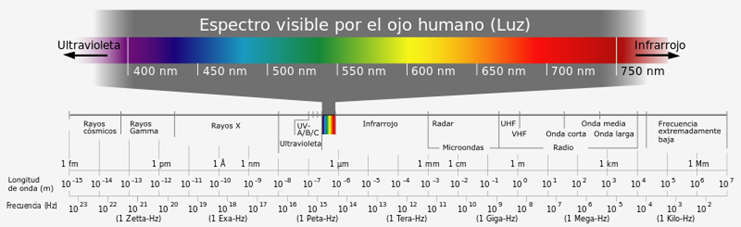
\includegraphics[width=5in]{1_espectro.png}
\end{center}
\caption{Espectro electromagnético}
\end{figure}

\\

 En este tutorial se explicará paso a paso cómo obtener imágenes de los satélites (Moderate-Resolution Imaging Spectroradiometer) MODIS y LANDSAT 8. Posteriormente cómo visualizarlas. El satélite MODIS capta información en 36 bandas del espectro electromagnético de 0.4 $\mu$m a 14.4 $\mu$m con resolución espacial (pixel) variante (2 bandas a 250m, 5 bandas a 500m y 29 bandas a 1km). El satélite Landsat 8 es el lanzamiento más reciente del programa Landsat. Capta información en 11 bandas del espectro, de 0.4 $\mu$m a 11.5 $\mu$m con una resolución espacial variante (8 bandas a 30m, 1 a 15m y 2 a 100m).

\newpage

Cada banda corresponde a un cierto "`color"' y más aún, a un cierto comportamiento físico determinado por cómo cierto terreno, y los objetos que allí se encuentran, reflejan la energía solar.

\\

\begin{figure}[h!]
\begin{center}
\leavevmode
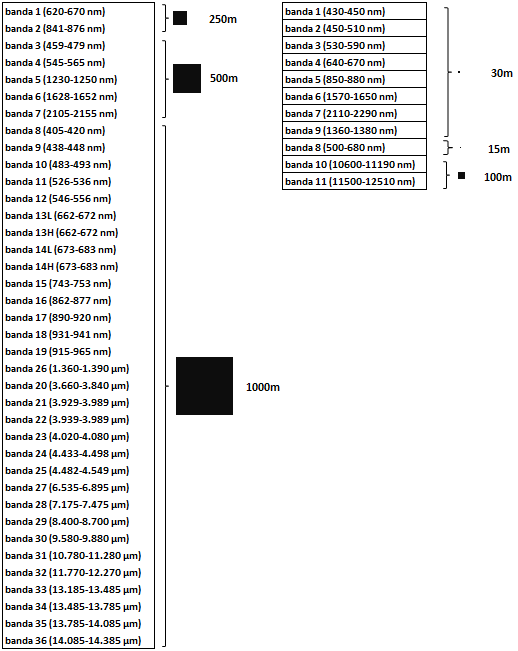
\includegraphics[width=4in]{2_bandas_modis_landsat.png}
\end{center}
\caption{Comparación bandas y tamaños de pixel: MODIS (izquierda) y Landsat 8 (derecha)}
\end{figure}

\newpage

\section{¿Por qué imágenes satelitales?}

Es importante recalcar que la utilidad de la información generada por estos satélites (imágenes) recae en que no sólo generan un modelo visual del lugar que están tomando, como lo hace una fotografía, si no que proveen de información física de los objetos que allí se encuentran. Distintos cuerpos, dependiendo de su naturaleza, reflejan la luz solar de distinta manera y en distintas intensidades.

\\
\begin{figure}[h!]
\begin{center}
\leavevmode
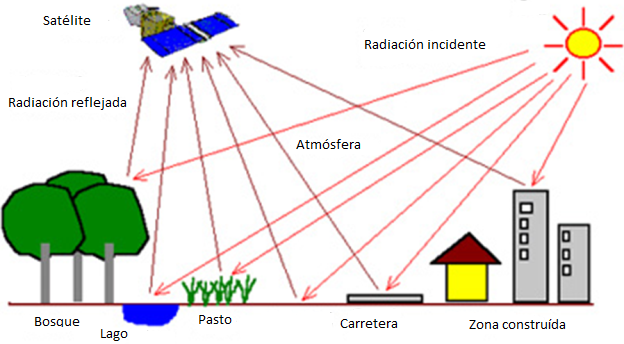
\includegraphics[width=4in]{3_sol_satelites.png}
\end{center}
\caption{Interacción: luz solar - atmósfera - terreno - atmósfera - satélite}
\end{figure}
\\

Por ejemplo es bien sabido que a muchas plantas las vemos verdes. Esto es resultado directo de que las hojas de estas plantas absorben más la parte de la luz solar que corresponde con el rojo y el azul puesto que utilizan esta energía en particular para llevar a cabo la fotosíntesis y alimentarse. Reflejan el verde por lo que lo que reciben nuestros ojos desde ellas nos hace visualizarlas en tonalidades de este color.


\\
\begin{figure}[h!]
\begin{center}
\leavevmode
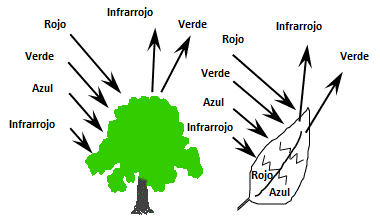
\includegraphics[width=3in]{4_plantas.png}
\end{center}
\caption{¿Por qué vemos verdes a las plantas?}
\end{figure}
\\

\newpage

De hecho, el concepto de "`color de un objeto"', por ejemplo una planta, es curioso.  Las plantas son del color del tipo luz que no abosorben, en este caso luz verde. Las plantas en realidad reflejan más la luz que correspondo al espectro infrarrojo, pero como se mostró en la figura 1.1, el ojo humano no es capaz de distinguir esta energía. Si pudiéramos ver "`en infrarrojo"' veríamos a las plantas infrarrojas. 





\chapter{Im\'agenes satelitales}
\section{Adquisición de imágenes}

En esta sección se darán instrucciones paso a paso sobre cómo obtener imágenes de los sensores MODIS y de las misiones Landsat. Hay múltiples maneras de conseguirlas desde utilizando portales web con interfases gráficas para este propísito hasta programando una conexión directa con los espacios de almacenamiento (File Transfer Protocol, FTPs) donde están albergadas las imágenes. Por ejemplo en servidores de la NASA. Se debe hacer hincapié en que, aunque está sujeto al objetivo del estudio, obtener imágenes satelitales puede ser una tarea ardua por la cantidad de datos que esto implica. 

\subsection{Landsat}

La manera más común en que se puede acceder a la colección completa de Landsat es en la plataforma EarthExplorer, puede hacer click en el siguiente link para entrar a esta plataforma: 

\\
\begin{center}
\url{<http://earthexplorer.usgs.gov/>}
\end{center}
\\

\\

\begin{figure}[h!]
\begin{center}
\leavevmode
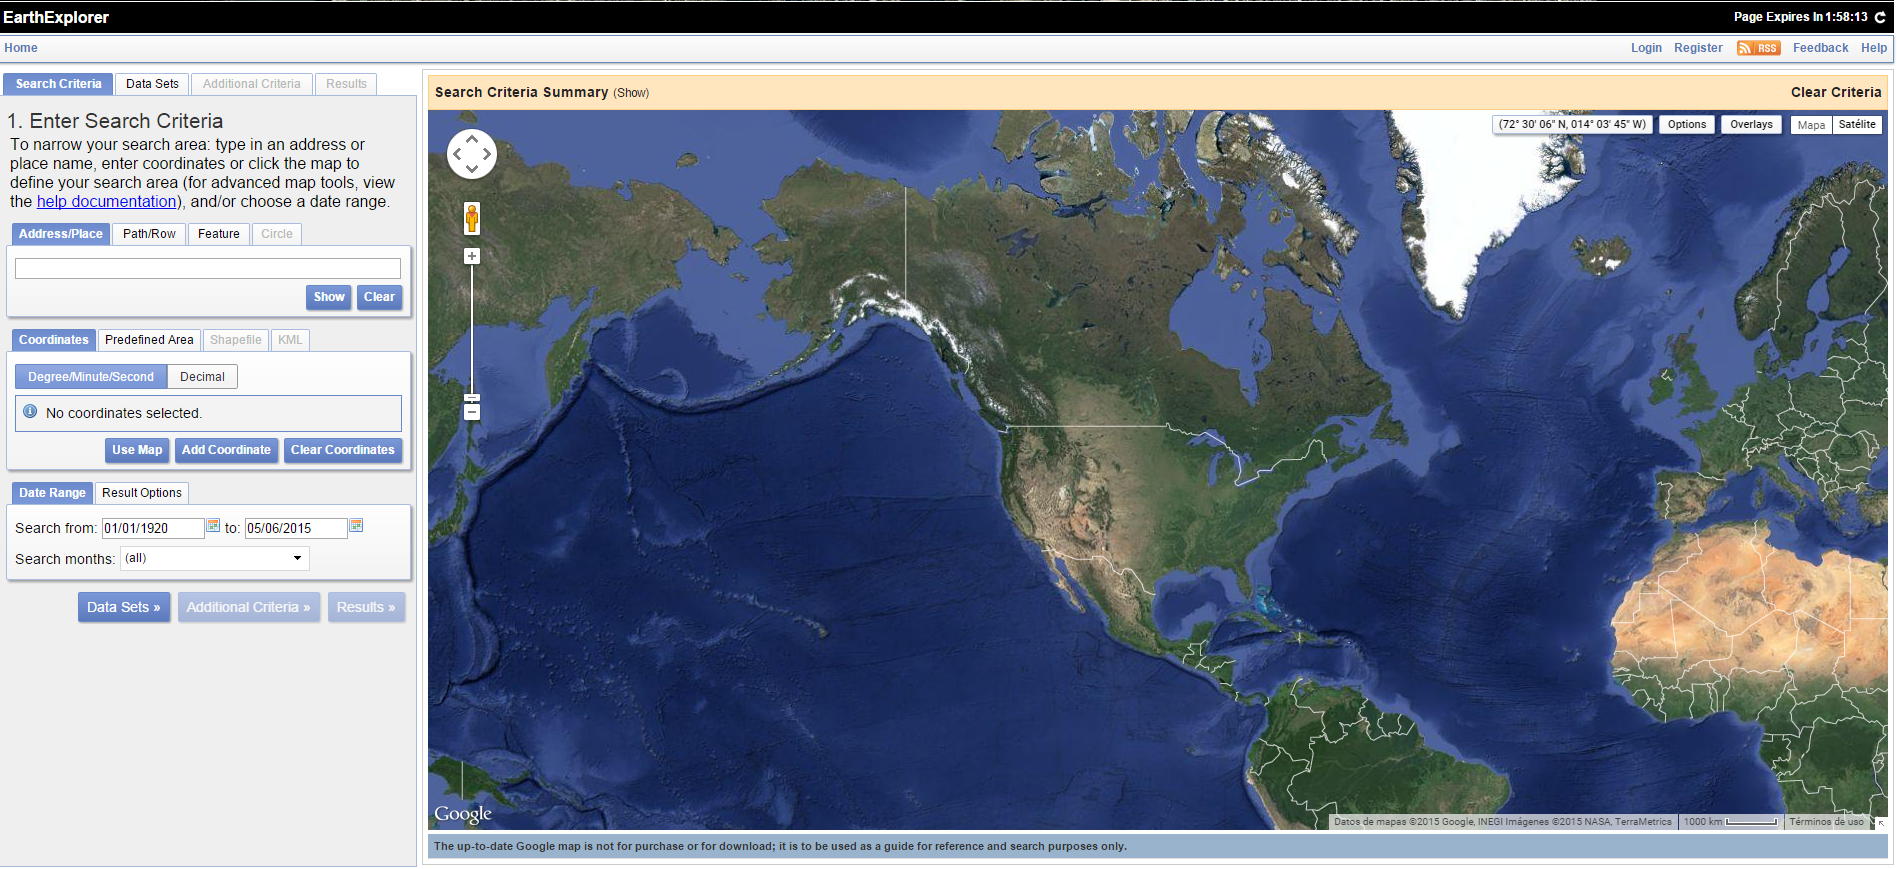
\includegraphics[width=6in]{5_earthexplorer.png}
\end{center}
\caption{Pantalla principal del portal EarthExplorer}
\end{figure}

\\

Primero debes de crear una cuenta en el portal. Sólo así podrás solicitar datos Landsat. Una vez que has llevado a cabo el proceso de registro podrás entrar a la plataforma con tus credenciales (nombre de usuario//contraseña). Cada imagen Landsat se encuentra sobre una cuadrícula que cubre al mundo. Cada uno de estos cuadros se llaman "`escenas"' y en ellas se encuentra toda una historia de adquisiciones de imágenes Landsat. Por ejemplo, en la figura 2.2 se muestra la cantidad de imágenes por escena para México tomadas en el año 2000.

\\

\begin{figure}[h!]
\begin{center}
\leavevmode
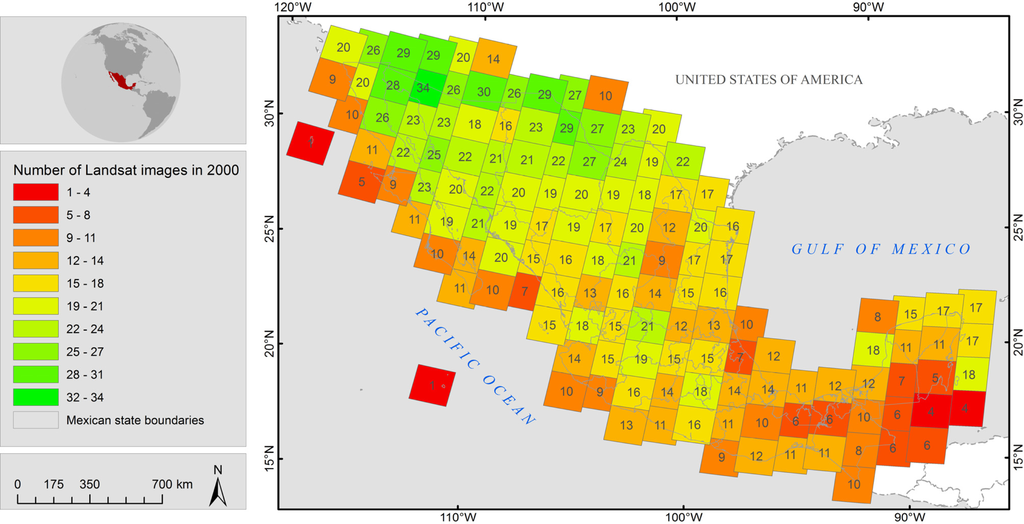
\includegraphics[width=5in]{6_escenas_landsat.png}
\end{center}
\caption{Imágenes por escena, año 2000}
\end{figure}

\\

Como se podrá observar, Landsat es uno de los múltiples conjuntos de datos que se pueden obtener en esta plataforma. También se ve que existen muchísimas maneras para hacer búsquedas en las colecciones para seleccionar los datos que cumplan con las características deseadas (localización espacial, fechas de adquisición, etc). Para generar una orden de datos puedes, por poner un ejemplo, subir una lista de escenas. Esta lista es un simple archivo de texto con un ID de esecna por renglón(eg: LT52302701999134). También puedes seleccionar una región utilizando el "`Search Criteria"' y utilizando la opción "`coordinates"' (figura 2.3). Se puede sencillamente mover los extremos de la región de interés en el mapa utilizando el mouse, por ejemplo envolviendo al estado de Veracruz.\\

Una vez elegida la región de interés de una manera u otra se debe de seleccionar las colecciones que se van a ubicar en tal región. Esto se hace utilizando la pestaña de "`Data sets"'. Por ejemplo si buscamos imágenes de la colección \textit{L7 ETM+ SLC-on (1999-2003)} obtenemos una lista de imágenes encontradas con tales características. Incluso se pueden visualizar en el mapa mismo apretando el ícono de visualización (figura 2.4). 

\newpage

\\

\begin{figure}[h!]
\begin{center}
\leavevmode
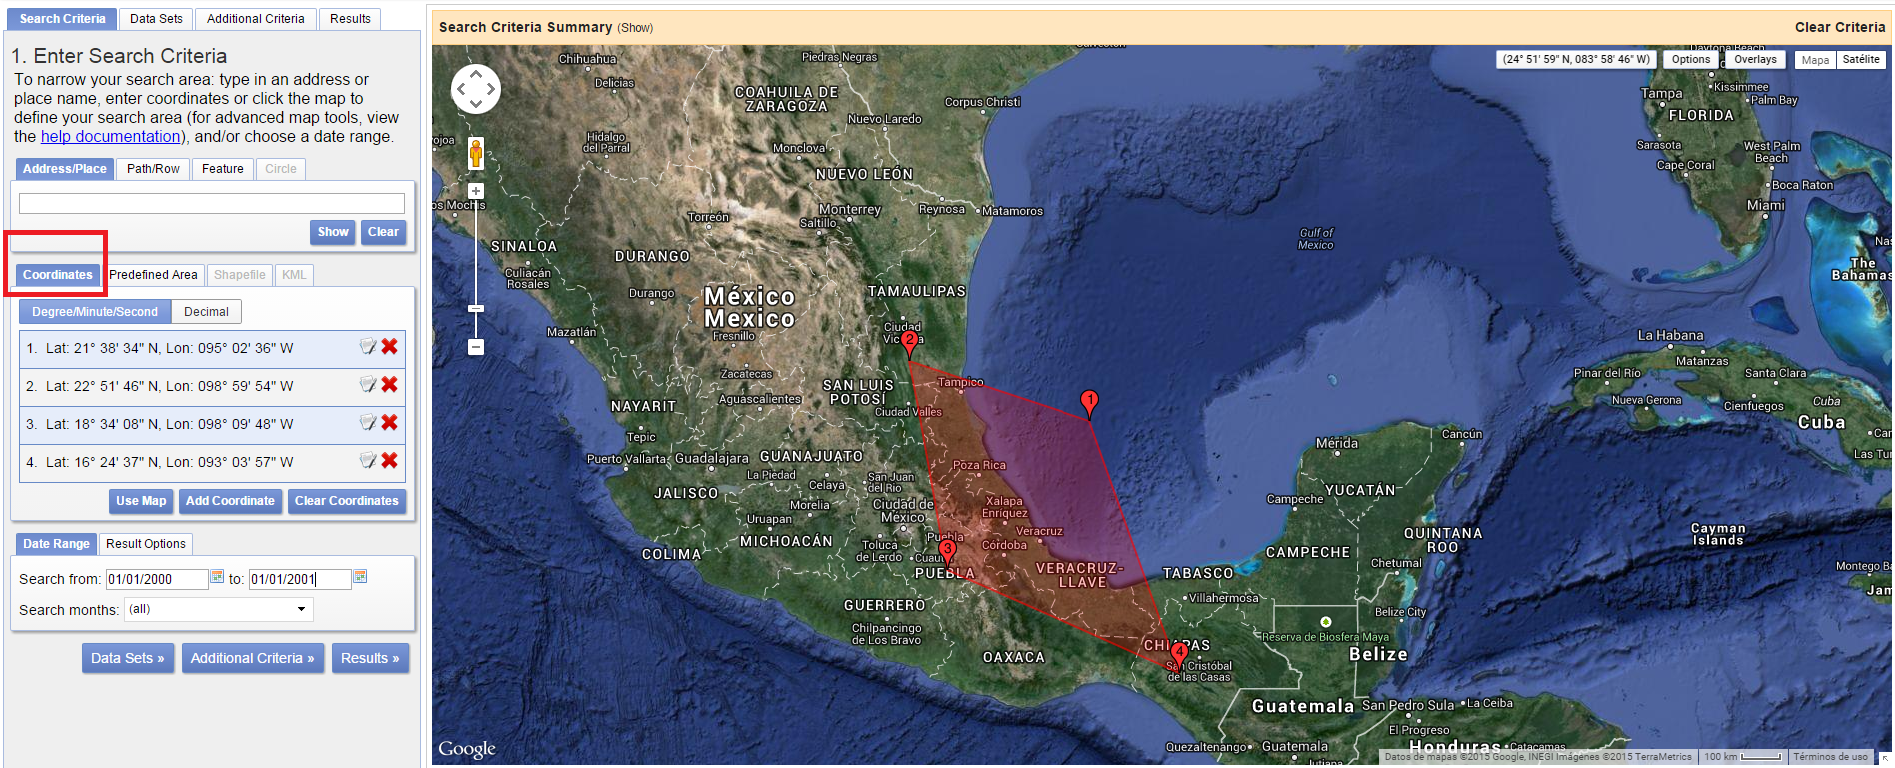
\includegraphics[width=6in]{7_veracruz.png}
\end{center}
\caption{Región de interés: Veracruz}
\end{figure}

\\



\\

\begin{figure}[h!]
\begin{center}
\leavevmode
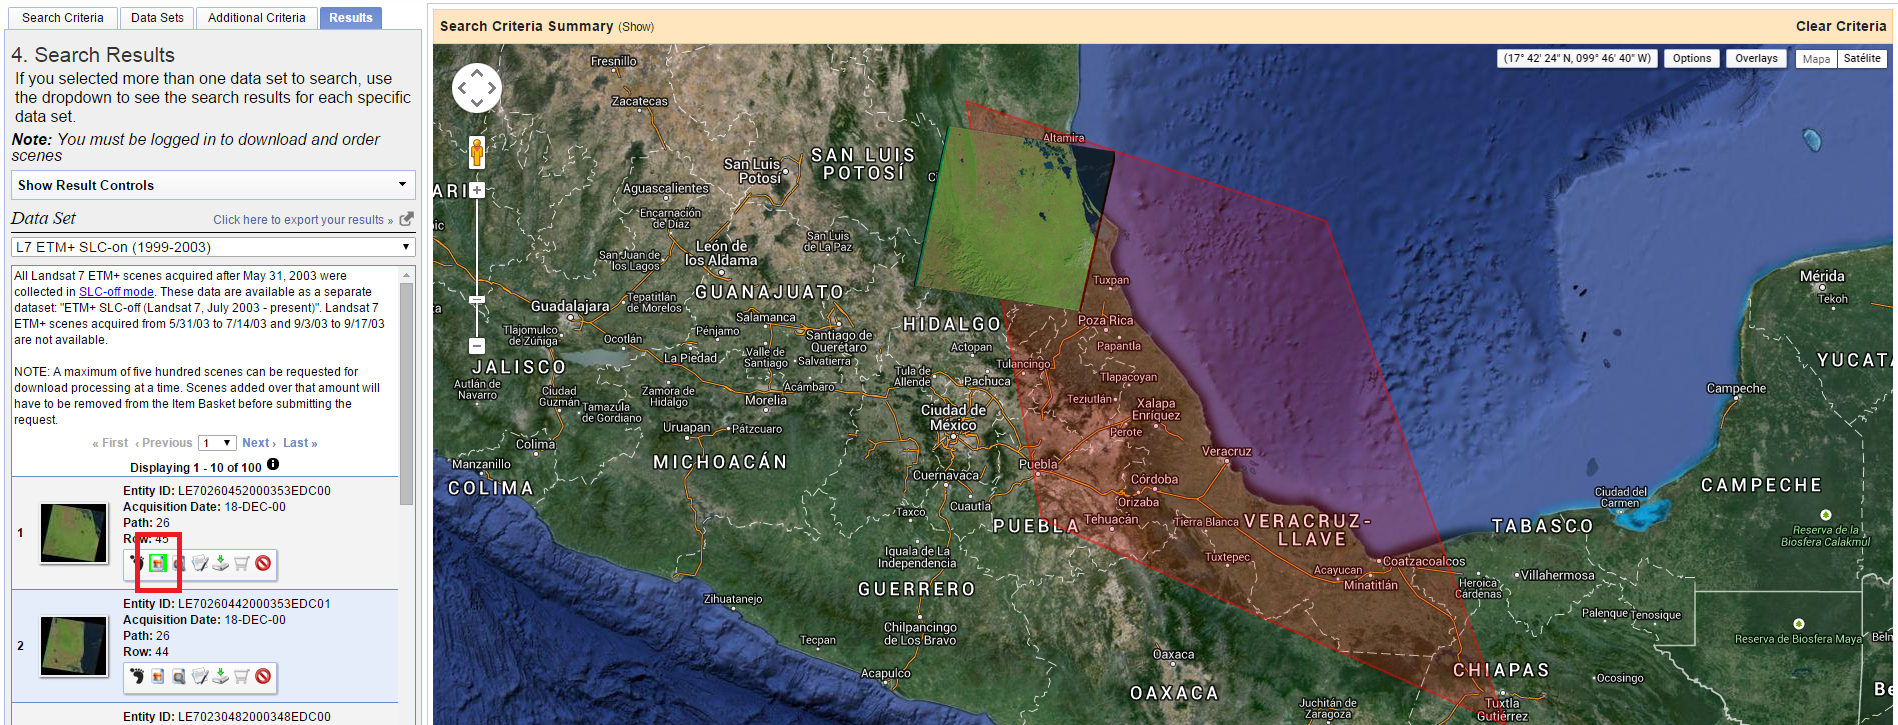
\includegraphics[width=6in]{8_overlay.png}
\end{center}
\caption{Imagen Landsat sobre Veracruz}
\end{figure}

\\

Ahora se debe pedir que la orden se pre-procese. Una vez que esto se lleva a cabo se recibirá un correo por parte de ESPA notificando que esto se realizacó con éxito y se podrá proceder a descargar la información. Como ya se mencionó, esto puede ser una tarea pesada por lo que se recomienda utilizar un manejador de descargas por ejemplo:

\begin{itemize}
	\item El Bulk Download Application (el manual será incluído con este tutorial)
	\item El complemento DownloadThemAll para firefox
\end{itemize}

\newpage

\subsection{MODIS}

Los servidores de la NASA donde se albergan los productos MODIS están abiertos. Incluso se podría bajar los datos manualmente:

\\
\begin{center}
\url{<http://e4ftl01.cr.usgs.gov/MOLT/>}
\end{center}
\\

Esto naturalmente resulta bastante confuso. Hay que entender varias cosas antes de adquirir imágenes MODIS. Primero, se procesan y ofrecen una gran cantidad de productos MODIS. En el siguiente link se puede revisar una tabla con cada uno de los productos disponibles:

\\
\begin{center}
\url{<https://lpdaac.usgs.gov/products/modis_products_table>}
\end{center}
\\

Cada uno tiene una respectiva clave ("`Short Name"'), en la tabla también se encuentran características básicas de los productos, la resolución temporal (periodicidad con la que existen, la resolución espacial, etc). Para más detalles se puede hacer click en los "`Short name"' y se accederá a una página con información técnica detallada del producto en cuestión. \\

Una vez elegido el producto se debe decidir qué imágenes se quieren obtener. Como sucede con Landsat, las imágenes MODIS también se encuentran sobre una cuadrícula sobre el mundo. Esta cuadrícula viene descrita por coordenadas horizontales y verticales (figura 2.5). 

\\
\begin{figure}[h!]
\begin{center}
\leavevmode
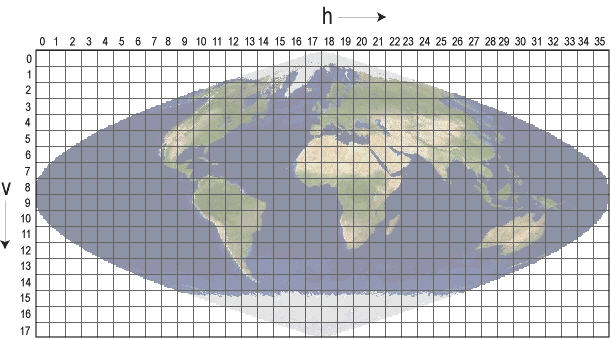
\includegraphics[width=4in]{9_modis_cuadricula.png}
\end{center}
\caption{Escenas MODIS}
\end{figure}
\\

Como con base en este mapa puede resultar muy difícil encontrar las coordenadas horizontales y verticales para regiones de interés, por ejemplo el estado de Veracruz, se incluye un archivo KMZ que se puede abrir en google earth para explorar las escenas MODIS con facilidad: MODISescenas.kmz . \\

Una vez encontradas las coorenadas horizontales y verticales de las escenas MODIS que incluyen a la región de interés estamos listos para adquirir las imágenes. Para este propósito se utilizará el languaje de programación R. Utilizando este lenguaje nos conectaremos diréctamente a los servidores de la NASA para luego bajar los archivos deseados.\\

Se requieren los siguientes \textbf{paquetes de R}:
\\ 

\begin{itemize}
	\item sp
	\item raster
	\item rgdal
	\item RCurl
	\item mail
	\item lubridate
	\item mapdata
	\item rgeos
	\item MODIS 
	
\end{itemize}

El paquete MODIS se debe obtener se puede bajar e instalar directamente de un zip o utilizar el commando indicado, figura 2.6.

\\
\begin{figure}[h!]
\begin{center}
\leavevmode
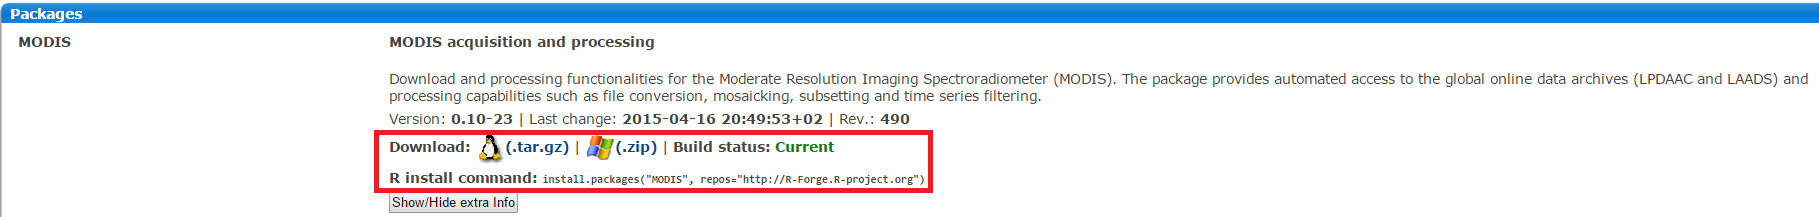
\includegraphics[width=6in]{10_modispackage.png}
\end{center}
\caption{Paquete de R: MODIS}
\end{figure}
\\

Otros requerimientos son:
\\

\textbf{Modis reprojection tool}: \url{<https://lpdaac.usgs.gov/tools/modis_reprojection_tool>}
\\
\begin{enumerate}
	\item 1.	Si ya se tenía instalado, quitar por complete el folder viejo MRT. Luego ir a System $\rightarrow$ Advanced $\rightarrow$ Environment Variables, y borrar todas las variables relacionadas con MRT de la ventana superior. 
	\item 2. Instalar/reinstalar MRT. Asegurarse que este se instala en c:\textbackslash{}Modis. 
	\item 3. Después de la instalación, ir nuevamente a las Environment Variables y en la ventana sueperior editar las tres entradas: 
	
	\begin{itemize}
		\item MRTDATADIR  c:\textbackslash{}Modis\textbackslash{}data 
		\item MRT$_$HOME    c:\textbackslash{}Modis 
		\item PATH        c: \textbackslash{}Modis\textbackslash{}bin 

	\end{itemize}
\end{enumerate}
\\

\textbf{Java}: \url{<https://www.java.com/es/download/>}\\
\\

Una vez que se tienen todos los requisitos se utiliza el script: bajarmodis.R donde deben elegir todos los parámetros de la descarga. Coordenadas de las escenas, producto a bajar, remuestreo, reproyección, etc de la información MODIS. El script viene comentado pero se debe leer con cuidado para bajar exactamente lo que se desea. Esto es, se debe elegir bien el producto y las fechas deseadas. Por otra parte se deben elegir bien las paths de salida de los productos procesados. También el tamaño correspondiente al producto, línea 105. 

%\chapter{Tareas a realizar}
%\section{Adquisición de imágenes}

En esta sección se darán instrucciones paso a paso sobre cómo obtener imágenes de los sensores MODIS y de las misiones Landsat. Hay múltiples maneras de conseguirlas desde utilizando portales web con interfases gráficas para este propísito hasta programando una conexión directa con los espacios de almacenamiento (File Transfer Protocol, FTPs) donde están albergadas las imágenes. Por ejemplo en servidores de la NASA. Se debe hacer hincapié en que, aunque está sujeto al objetivo del estudio, obtener imágenes satelitales puede ser una tarea ardua por la cantidad de datos que esto implica. 

\subsection{Landsat}

La manera más común en que se puede acceder a la colección completa de Landsat es en la plataforma EarthExplorer, puede hacer click en el siguiente link para entrar a esta plataforma: 

\\
\begin{center}
\url{<http://earthexplorer.usgs.gov/>}
\end{center}
\\

\\

\begin{figure}[h!]
\begin{center}
\leavevmode
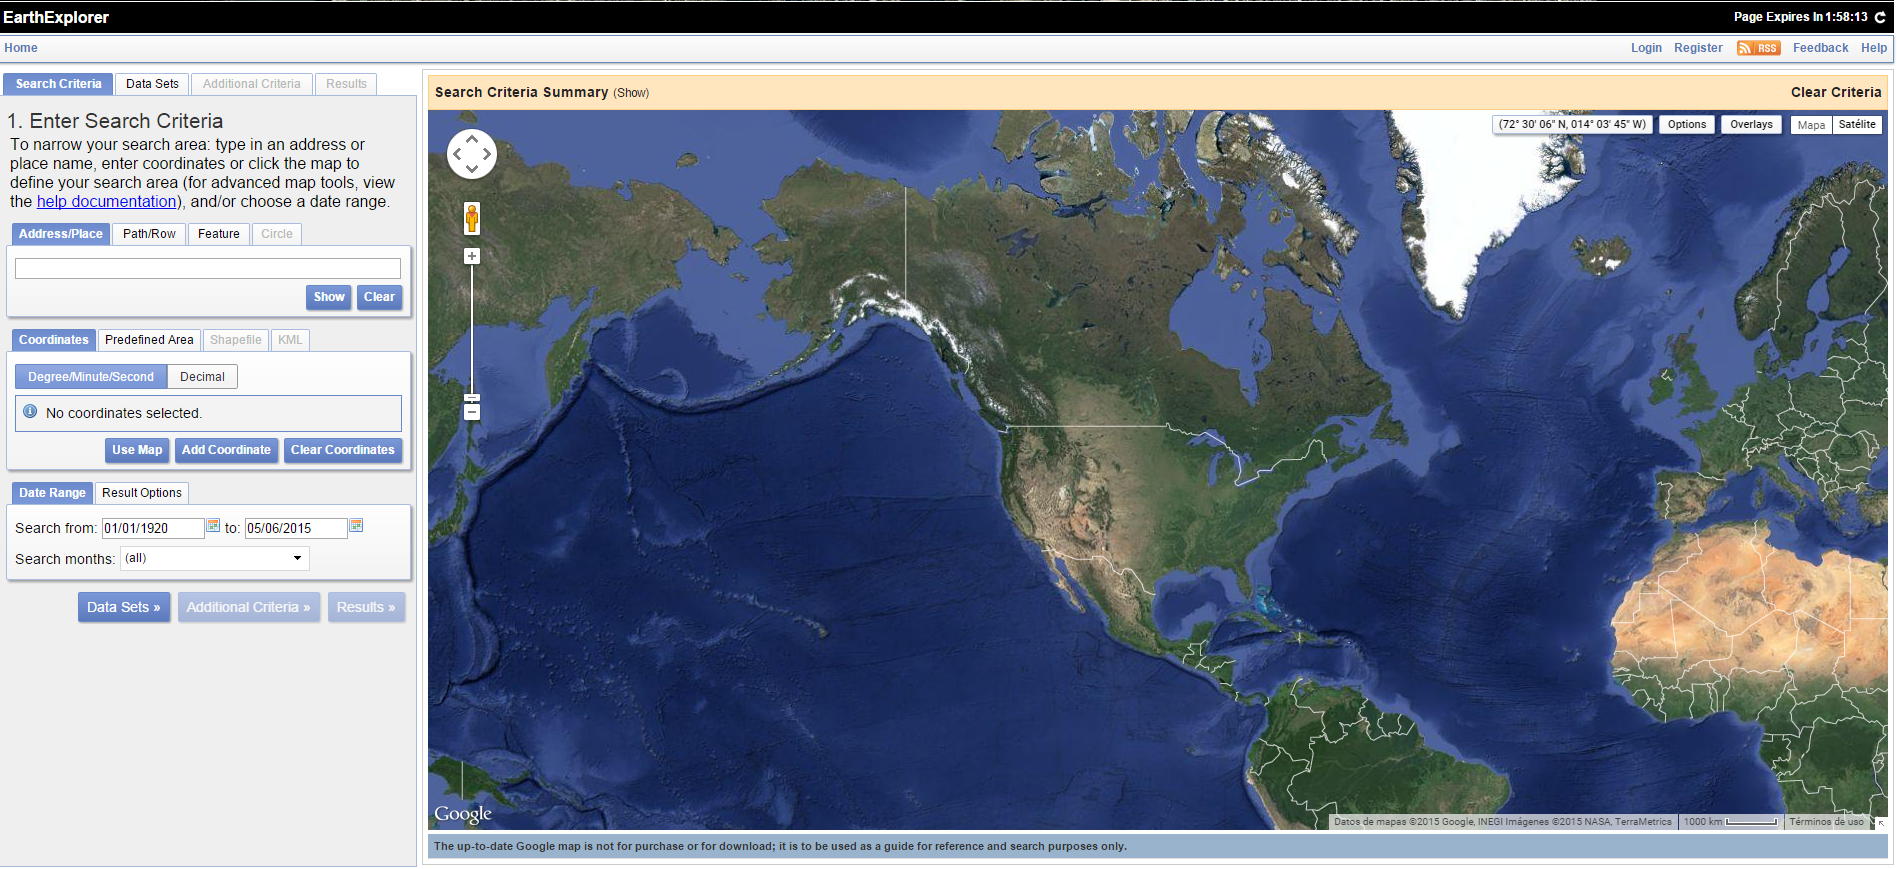
\includegraphics[width=6in]{5_earthexplorer.png}
\end{center}
\caption{Pantalla principal del portal EarthExplorer}
\end{figure}

\\

Primero debes de crear una cuenta en el portal. Sólo así podrás solicitar datos Landsat. Una vez que has llevado a cabo el proceso de registro podrás entrar a la plataforma con tus credenciales (nombre de usuario//contraseña). Cada imagen Landsat se encuentra sobre una cuadrícula que cubre al mundo. Cada uno de estos cuadros se llaman "`escenas"' y en ellas se encuentra toda una historia de adquisiciones de imágenes Landsat. Por ejemplo, en la figura 2.2 se muestra la cantidad de imágenes por escena para México tomadas en el año 2000.

\\

\begin{figure}[h!]
\begin{center}
\leavevmode
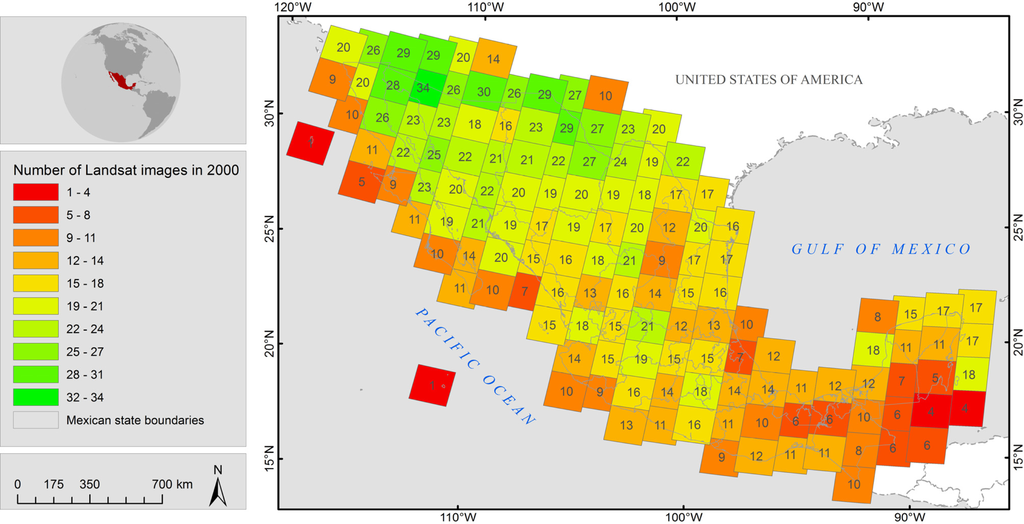
\includegraphics[width=5in]{6_escenas_landsat.png}
\end{center}
\caption{Imágenes por escena, año 2000}
\end{figure}

\\

Como se podrá observar, Landsat es uno de los múltiples conjuntos de datos que se pueden obtener en esta plataforma. También se ve que existen muchísimas maneras para hacer búsquedas en las colecciones para seleccionar los datos que cumplan con las características deseadas (localización espacial, fechas de adquisición, etc). Para generar una orden de datos puedes, por poner un ejemplo, subir una lista de escenas. Esta lista es un simple archivo de texto con un ID de esecna por renglón(eg: LT52302701999134). También puedes seleccionar una región utilizando el "`Search Criteria"' y utilizando la opción "`coordinates"' (figura 2.3). Se puede sencillamente mover los extremos de la región de interés en el mapa utilizando el mouse, por ejemplo envolviendo al estado de Veracruz.\\

Una vez elegida la región de interés de una manera u otra se debe de seleccionar las colecciones que se van a ubicar en tal región. Esto se hace utilizando la pestaña de "`Data sets"'. Por ejemplo si buscamos imágenes de la colección \textit{L7 ETM+ SLC-on (1999-2003)} obtenemos una lista de imágenes encontradas con tales características. Incluso se pueden visualizar en el mapa mismo apretando el ícono de visualización (figura 2.4). 

\newpage

\\

\begin{figure}[h!]
\begin{center}
\leavevmode
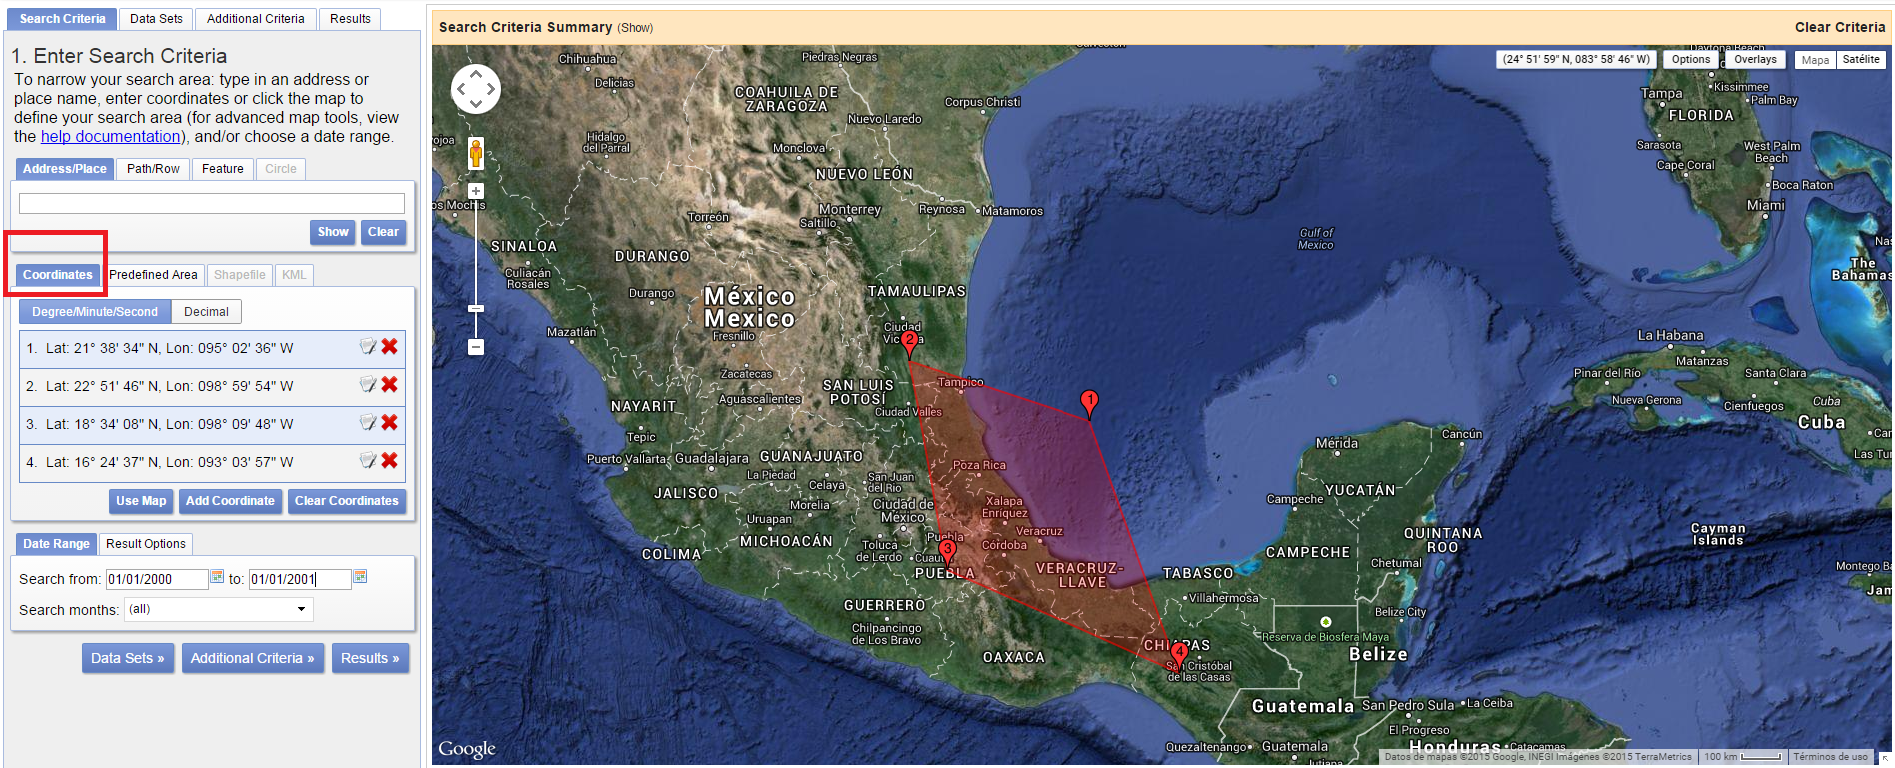
\includegraphics[width=6in]{7_veracruz.png}
\end{center}
\caption{Región de interés: Veracruz}
\end{figure}

\\



\\

\begin{figure}[h!]
\begin{center}
\leavevmode
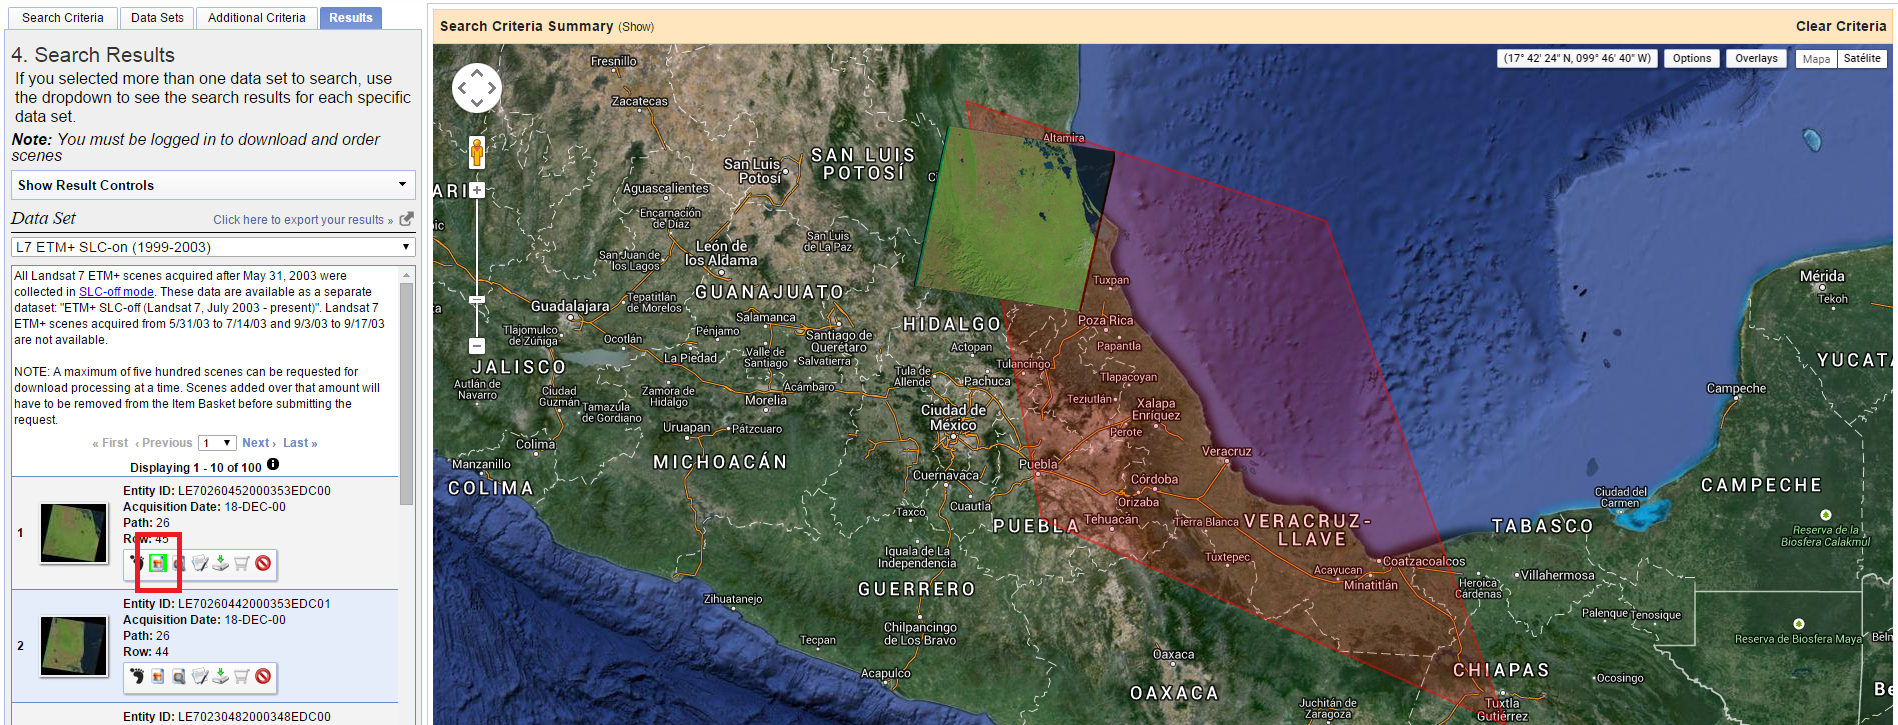
\includegraphics[width=6in]{8_overlay.png}
\end{center}
\caption{Imagen Landsat sobre Veracruz}
\end{figure}

\\

Ahora se debe pedir que la orden se pre-procese. Una vez que esto se lleva a cabo se recibirá un correo por parte de ESPA notificando que esto se realizacó con éxito y se podrá proceder a descargar la información. Como ya se mencionó, esto puede ser una tarea pesada por lo que se recomienda utilizar un manejador de descargas por ejemplo:

\begin{itemize}
	\item El Bulk Download Application (el manual será incluído con este tutorial)
	\item El complemento DownloadThemAll para firefox
\end{itemize}

\newpage

\subsection{MODIS}

Los servidores de la NASA donde se albergan los productos MODIS están abiertos. Incluso se podría bajar los datos manualmente:

\\
\begin{center}
\url{<http://e4ftl01.cr.usgs.gov/MOLT/>}
\end{center}
\\

Esto naturalmente resulta bastante confuso. Hay que entender varias cosas antes de adquirir imágenes MODIS. Primero, se procesan y ofrecen una gran cantidad de productos MODIS. En el siguiente link se puede revisar una tabla con cada uno de los productos disponibles:

\\
\begin{center}
\url{<https://lpdaac.usgs.gov/products/modis_products_table>}
\end{center}
\\

Cada uno tiene una respectiva clave ("`Short Name"'), en la tabla también se encuentran características básicas de los productos, la resolución temporal (periodicidad con la que existen, la resolución espacial, etc). Para más detalles se puede hacer click en los "`Short name"' y se accederá a una página con información técnica detallada del producto en cuestión. \\

Una vez elegido el producto se debe decidir qué imágenes se quieren obtener. Como sucede con Landsat, las imágenes MODIS también se encuentran sobre una cuadrícula sobre el mundo. Esta cuadrícula viene descrita por coordenadas horizontales y verticales (figura 2.5). 

\\
\begin{figure}[h!]
\begin{center}
\leavevmode
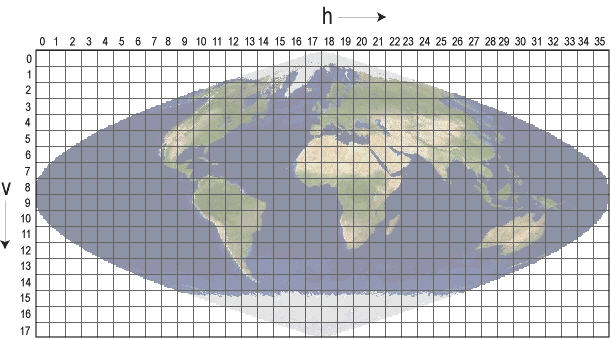
\includegraphics[width=4in]{9_modis_cuadricula.png}
\end{center}
\caption{Escenas MODIS}
\end{figure}
\\

Como con base en este mapa puede resultar muy difícil encontrar las coordenadas horizontales y verticales para regiones de interés, por ejemplo el estado de Veracruz, se incluye un archivo KMZ que se puede abrir en google earth para explorar las escenas MODIS con facilidad: MODISescenas.kmz . \\

Una vez encontradas las coorenadas horizontales y verticales de las escenas MODIS que incluyen a la región de interés estamos listos para adquirir las imágenes. Para este propósito se utilizará el languaje de programación R. Utilizando este lenguaje nos conectaremos diréctamente a los servidores de la NASA para luego bajar los archivos deseados.\\

Se requieren los siguientes \textbf{paquetes de R}:
\\ 

\begin{itemize}
	\item sp
	\item raster
	\item rgdal
	\item RCurl
	\item mail
	\item lubridate
	\item mapdata
	\item rgeos
	\item MODIS 
	
\end{itemize}

El paquete MODIS se debe obtener se puede bajar e instalar directamente de un zip o utilizar el commando indicado, figura 2.6.

\\
\begin{figure}[h!]
\begin{center}
\leavevmode
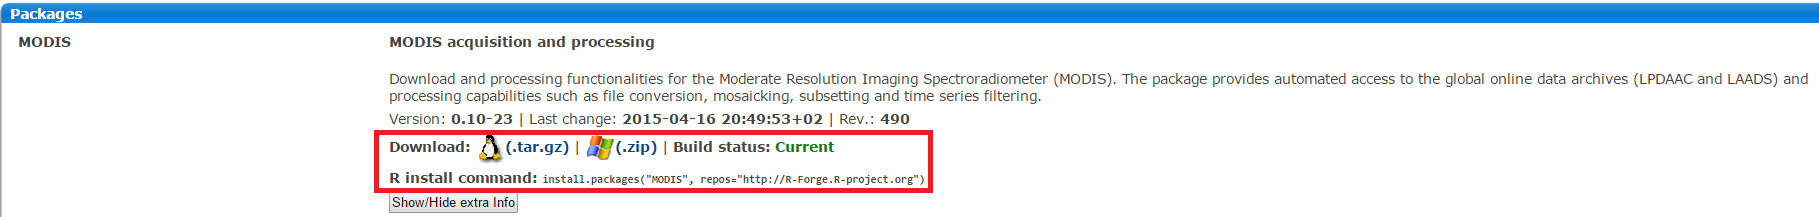
\includegraphics[width=6in]{10_modispackage.png}
\end{center}
\caption{Paquete de R: MODIS}
\end{figure}
\\

Otros requerimientos son:
\\

\textbf{Modis reprojection tool}: \url{<https://lpdaac.usgs.gov/tools/modis_reprojection_tool>}
\\
\begin{enumerate}
	\item 1.	Si ya se tenía instalado, quitar por complete el folder viejo MRT. Luego ir a System $\rightarrow$ Advanced $\rightarrow$ Environment Variables, y borrar todas las variables relacionadas con MRT de la ventana superior. 
	\item 2. Instalar/reinstalar MRT. Asegurarse que este se instala en c:\textbackslash{}Modis. 
	\item 3. Después de la instalación, ir nuevamente a las Environment Variables y en la ventana sueperior editar las tres entradas: 
	
	\begin{itemize}
		\item MRTDATADIR  c:\textbackslash{}Modis\textbackslash{}data 
		\item MRT$_$HOME    c:\textbackslash{}Modis 
		\item PATH        c: \textbackslash{}Modis\textbackslash{}bin 

	\end{itemize}
\end{enumerate}
\\

\textbf{Java}: \url{<https://www.java.com/es/download/>}\\
\\

Una vez que se tienen todos los requisitos se utiliza el script: bajarmodis.R donde deben elegir todos los parámetros de la descarga. Coordenadas de las escenas, producto a bajar, remuestreo, reproyección, etc de la información MODIS. El script viene comentado pero se debe leer con cuidado para bajar exactamente lo que se desea. Esto es, se debe elegir bien el producto y las fechas deseadas. Por otra parte se deben elegir bien las paths de salida de los productos procesados. También el tamaño correspondiente al producto, línea 105. 

\end{document}